\documentclass[a4paper]{article}

\usepackage[english]{babel}
\usepackage[utf8]{inputenc}
\usepackage{amsmath}
\usepackage{graphicx}
\usepackage[colorinlistoftodos]{todonotes}

\title{Behaviour Dynamics in Social Networks - Assignment 3}

\author{Maria Hotoiu, Federico Tavella}

\date{\today}

\begin{document}
\maketitle

\begin{abstract}
As the first step of this assignment, you are asked to model the example of temporal-causal network
model described in Chapter2. The following figure shows the graphical conceptual representation of
this model. You can use the Excel template created for this modeling purpose (available on Blackboard
of the course). For more information about this model, please read Section 4 of Chapter 2.
\end{abstract}

\section{Simulation result}

\begin{figure}[!htpb]
\center
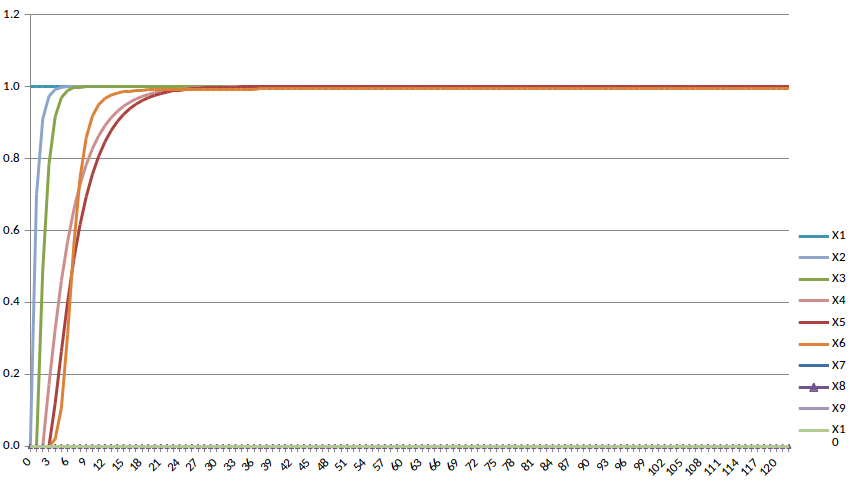
\includegraphics[width=\textwidth]{res/img/results}
\caption{Simulation result}
\label{fig:simulation_result}
\end{figure}

\section{Physical action}

The value of $es_a$ is going above 0.5 between 7 and 8 seconds. In order to delay the physical response, we should change the speed factor (e.g. $\eta_{es_{a}} = 0.1$). If we want the value of $es_{a}$ to overcome 0.5 after 20 seconds, we should use $\eta_{es_{a}} = 0.05$.

\begin{figure}[!htpb]
\center
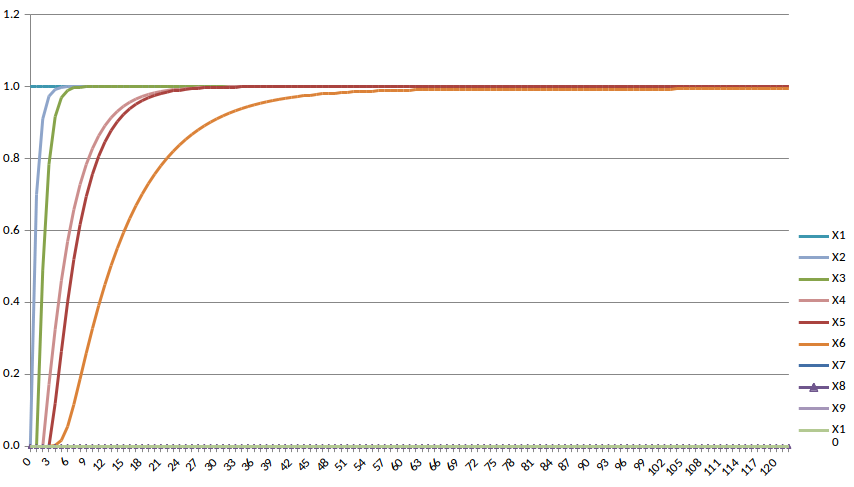
\includegraphics[width=\textwidth]{res/img/results_speed_factor}
\caption{Simulation result with $\eta_{es_{a}} = 0.05$}
\label{fig:simulation_result_speed_factor}
\end{figure}

\section{Smoother curves}

In order to obtain smoother curves, we have to change the $\Delta t$ to a smaller value.

\begin{figure}[!htpb]
\center
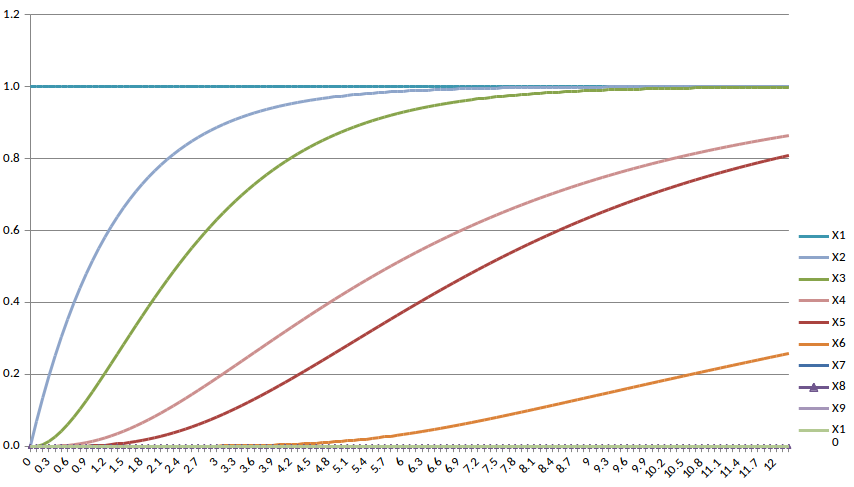
\includegraphics[width=\textwidth]{res/img/results_delta_t}
\caption{Simulation result with $\Delta t = 0.1$}
\label{fig:simulation_result_delta_t}
\end{figure}

Now, the value of $es_{a}$ is becoming higher than 0.5 after 7.2 seconds, which is between 7 and 8, as for Q2.
$\Delta t$ does not affect how fast the values are changing, it only changes the frequency of observations. On the other hand, the speed factor influences how rapidly the values are varying. Moreover, the $\Delta t$ is shared for the whole model, while the speed factor is characteristic to each node.

\section{Tuning $es_{a}$}

The closer we could get to the empirical values for $es_{a}$ is using the following parameters: $\eta_{es_{a}} = 0.33,$ $\sigma_{es_{a}} = 62$ and $\tau_{es_{a}} = 0.948$. With these values, we obtain $es_{a}(t = 0) = 0$, $es_{a}(t = 15) = 0.114$ and $es_{a}(t = 30) = 0.946$.

\begin{figure}[!htpb]
\center
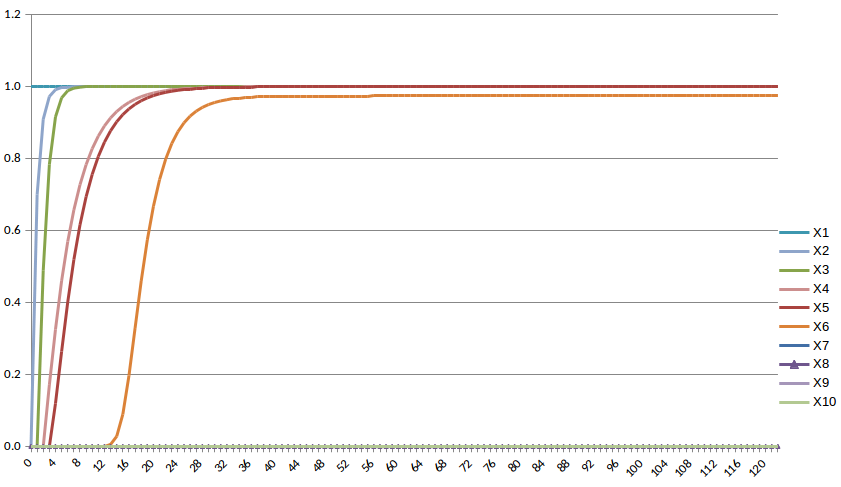
\includegraphics[width=\textwidth]{res/img/tuning}
\caption{Tuning of parameters for $es_{a}$}
\label{fig:tuning}
\end{figure}

\section{Real world scenarios}

Real world domains where we can have different $\Delta t$ for different processes to have a most accurate simulation: the first scenario is observing patients in a mental institute and the second one is.

\begin{enumerate}
\item We can have smaller $\Delta t$ when we need to check the changes of the values more often. For example, if we are studying a case where people with severe depression are concerned, we want to check the evolution of the emotions really often, otherwise we could not predict if they are going to hurt themselves. With a bigger $\Delta t$, we check the evolution of states less frequently. In this case, we can monitor people with OCD less frequently because they are less likely to be in danger.
\item 
\end{enumerate}

Two real world application domains for which one value of $\Delta t$ will make a most accurate simulation:

\begin{enumerate}
\item 
\item 
\end{enumerate}

\section{Comparision of $\Delta t$ and speed factor}

True sentences: (g). False sencences: all the other ones.
$\Delta t$ is only a property of the model: in reality, the process is continuous, while in a simulation it is discrete. On the other hand, the speed factor is a property of both real world and the model: all real life processes have a certain speed and to represent them we need to include the speed factor as a property of the model.



\end{document}
